\documentclass[10pt,a4paper]{article}
\usepackage[utf8]{inputenc}

% \usepackage{ngerman}  % german documents
\usepackage{graphicx}  % import graphics einbinden
\usepackage{listings}  % support source code listing
\usepackage{amsmath}  % math stuff
\usepackage{amssymb} % 
\usepackage{a4wide} % wide pages
\usepackage{fancyhdr} % nice headers
\usepackage{float}
\usepackage{longtable}
\usepackage{xcolor}
\usepackage{cite}
\usepackage{fancyhdr}
\usepackage{tabularx}
\usepackage{booktabs}
\usepackage{lscape}
\usepackage{gensymb}
\usepackage{textgreek}



% For bibliography in two columns
\usepackage{multicol}
\usepackage{etoolbox}

\usepackage[pdfpagemode=None, colorlinks=true,  % url coloring
linkcolor=blue, urlcolor=blue, citecolor=blue, plainpages=false, 
pdfpagelabels,unicode]{hyperref}

\definecolor{darkpastelgreen}{rgb}{0.01, 0.75, 0.24}
\definecolor{spirodiscoball}{rgb}{0.06, 0.75, 0.99}
\definecolor{smalt}{rgb}{0.0, 0.2, 0.6}
\definecolor{armygreen}{rgb}{0.29, 0.33, 0.13}
\definecolor{awesome}{rgb}{1.0, 0.13, 0.32}
\definecolor{bittersweet}{rgb}{1.0, 0.44, 0.37}
\definecolor{bananayellow}{rgb}{1.0, 0.88, 0.21}
\definecolor{blue}{rgb}{0.0, 0.0, 1.0}
\definecolor{red}{rgb}{1.0, 0.0, 0.0}
\definecolor{green}{rgb}{0.0, 1.0, 0.0}





\title{\Huge Bioinformatics Practicals In Sillico \\ \textbf{\normalsize BC-7107}}

%\raggedright
%
\includegraphics[width = 40mm]{img/unibe.png}\\[8ex]

\vfill
%set up names, matricle number, and email
\author{
	\noindent
	\begin{tabular}[t]{@{}l}
		\href{mailto:thibault.schowing@unifr.ch}{Thibault Schowing}\\
		\href{mailto:lio_roh@students.unibe.ch}{Lionel Rohner}\\
		\href{mailto:alain.rohrbasser.unifr.ch}{Alain Rohrbasser}\\
		\href{mailto:rares.cristea@unifr.ch}{Rares Cristea}
	\end{tabular}
		}

%\hfill
%\raisebox{\dimexpr.8\baselineskip-\height}{\includegraphics[width=32mm]{example-image}}


\begin{document}


\pagestyle{fancy}             % header
\setcounter{page}{1}

%lecture name
\newcommand{\lecture}{
	Bioinformatics Practicals In Sillico
}           

%assignment iteration
\newcommand{\assignment}{
	BC-7107
}


\setlength \headheight{25pt}
\fancyhead[R]{\begin{tabular}{r}\lecture \\ \assignment \end{tabular}}
\fancyhead[L]{HS-2019}


\part*{\Large Identification of $\Delta$TOM1 suppressors in \textit{S. Cerevisiae}}

\href{mailto:thibault.schowing@unifr.ch}{Thibault Schowing}, \href{mailto:lio_roh@students.unibe.ch}{Lionel Rohner},
\href{mailto:alain.rohrbasser.unifr.ch}{Alain Rohrbasser},
\href{mailto:rares.cristea@unifr.ch}{Rares Cristea}\\

\section*{\large Introduction}


The budding yeast \textit{Saccharomyces cerevisiae} (\textit{S.cerevisiae}) is a single-celled lower eukaryote belonging to the kingdom of fungi. Ever since its discovery, \textit{S.cerevisae} has nourished human advancements in the field of fermented food products, alcoholic beverages, and nowadays, the production of biofuel. Beyond its contributions to industrial fermentation, \textit{S.cerevisiae} has become one of the most popular model organism in eukaryotic biology, due to its simple cellular architecture, cheap maintenance cost, fast growth, and homologies to human cells \cite{botstein_yeast_2011}. Since the genome of \textit{S.cerevisiae} is fully sequenced, relatively small and virtually free of intronic DNA, this microorganism is ideally suited for genetic analyses.\\

\noindent In this project, we focused on identifying novel mutations that may suppress the phenotypic alteration caused by the deletion of the gene Trigger of mitosis, abbreviated \textit{TOM1}. \textit{TOM1} is a gene located on chromosome 4 and codes for a Hect-domain E3 ubiquitin ligase \cite{utsugi_yeast_1999}. Utsugi and colleagues found that mutations in the Hect-domain of \textit{TOM1}, which is necessary for thioester-bond formation with ubiquitin, or deletion of the entire gene rendered \textit{S.cerevisiae} unable to grow at high temperatures \cite{utsugi_yeast_1999}. The authors found that \textit{S.cerevisiae} with mutated \textit{TOM1} exhibited an abnormally large nucleus containing duplicated DNA, fragmented nucleoli, accumulation of poly(A)+RNA in the nucleus, and cell cycle arrest at G2/M, suggesting that the disruption of \textit{TOM1} had a severe impact on nuclear transport and cell division. Later it was shown that TOM1 was targeting DIA2 and CDC6 for proteasomal degradation during G1 and G2/M phases \cite{kim_hect_2012}, confirming that TOM1 is involved in the regulation of the cell cycle.\\

\noindent Furthermore, TOM1 has been found to play an integral role in the regulation of proteostasis by ubiquitinating highly basic histone proteins \cite{singh_histone_2009} and various unassembled ribosomal proteins of the large and small subunit (RPL and RPS, respectively)\cite{sung_conserved_2016}. This demonstrates that the deletion of \textit{TOM1} (termed \textit{$\Delta$TOM1}) has a highly pleiotropic effect on the phenotype of \textit{S.cerevisiae} under heat stress. To date, several extragenic suppressors of \textit{$\Delta$TOM1} have been identified that restore the ability of  \textit{S.cerevisiae} to grow at high temperatures, such as deletion of \textit{DIA2}\cite{kim_hect_2012}, overexpression of \textit{STM1}\cite{utsugi_high_1995}, as well as mutations in genes that are linked to down-regulation of the cAMP/PKA pathway \cite{sasaki_extragenic_2000}.The aim of this study was to identify potential new extragenic suppressors of \textit{$\Delta$TOM1} in six strains of  \textit{S.cerevisiae} that were derived from YDK1364. While YDK1364 is unable to grow under heat stress due to the deletion of \textit{TOM1}, the tested strains partially regained the ability to grow at high temperatures due to the accumulation of random mutations. The six strains were sequenced and potential mutations associated with the revertant phenotype were identified using a bioinformatic pipeline. We found one known suppressor of \textit{$\Delta$TOM1}, as well as some new candidates that were mostly associated with the \textit{RPL} and \textit{RPS} gene family. \\



\section*{\large Methods}

\paragraph{Sequencing and quality control of raw data} Yeast samples were sequenced by Illumina Sequencing Technology (Illumina, SanDiego, CA, USA). As high-throughput sequencing is not infallible and sequencing errors cannot be avoided, we used \href{http://www.bioinformatics.babraham.ac.uk/projects/fastqc/}{FastQC} to perform various quality checks of raw sequence data to ensure good quality and avoid biased data. Quality checks of FastQC, include sequence quality, GC content, failed base call content (N content), and k-mer content.



\paragraph{Quality control of reads} After the quality control check, \textit{trimmomatic}\cite{bolger_trimmomatic:_2014} was used with the parameters of MINLEN : 130 to trim down the bad quality ends of the reads, keeping at least 130bp of the trimmed read, and the parameter SLIDINGWINDOW:4:15, thus removing the reads that have an average base pair quality score lower than 15. To check the quality of the data after the trimming process, FastQC was used again on the filtered fasta files.

\paragraph{Sequence alignment against reference} The fasta files containing the filtered reads were mapped to the reference genome Assembly \href{https://www.ensembl.org/Saccharomyces_cerevisiae/Info/Index}{R64-1-1.92}. In a first step, the reference genome was indexed by the \textit{bwa} (Burrows-Wheeler Aligner) index tool\cite{li_fast_2010}. Subsequently, the \textit{bwa mem} tool was used to map the sequenced reads to the reference genome. The output files of the \textit{bwa} tool were then converted into SAM files\cite{li_sequence_2009}.
 
\paragraph{Variant calling and annotation}
First, \textit{SAMtools view}\cite{li_sequence_2009} was used to convert the SAM files into BAM files, which is a compressed binary format. Next, the BAM files were sorted using \textit{SAMtools sort}. This has been done using \textit{SAMtools mpileup}, that took our reference file, and the aligned BAM files as an input. Then the output file, a binary format of the \textit{Variant Calling Format} files (.bcf) was directly piped into \href{www.http://www.htslib.org/}{\textit{BCFtools}} to convert them into compressed vcf.gz files. This method was preferred considering the fact that our genome is a haploid yeast genome, and it does not need a complicated algorithm as used by the \href{https://software.broadinstitute.org/gatk/}{GATK4} pipeline. The \textit{Tabix}\cite{li_tabix:_2011} tool was used on the vcf files, in order to index them properly. Annotations of the variants was done by \href{http://snpeff.sourceforge.net/}{SnpEff} tool on the merged vcf files. The results were then visualized by either reading the vcf files in a spreadsheet or in IGV (\href{http://software.broadinstitute.org/software/igv/}{Integrative Genomics Viewer}).\\



\section*{\large Results}
We screened the \textit{S.cerevisae} samples T5, T6, T7 and T8 for interesting mutations that could potentially be responsible for reverting the heat-sensitive phenotype of \textit{$\Delta$TOM1} \textit{S.cerevisae} strains. The sample T5 contains only one haploid strain named YDK1364 and was used as a reference (Figure \ref{fig:yeastgrowth}). All strains found in T6 to T8 arose from the strain YDK1364 found in T5, but as mutations emerged in strains S1364-1 to S1364-8, these strains became more resistant to high-temperature stress (i.e. 37\degree C). Therefore, we excluded all mutations that co-occurred in T5 and any of the samples of interest T6 to T8. Since each of the samples is composed of two pooled haploid \textit{S.cerevisae} strains (Figure \ref{fig:yeastgrowth}), we excluded all homozygous mutations from further analysis, since it is highly unlikely that two strains have the same mutation suppressing the $\Delta$TOM1 heat sensitivity phenotype.

\begin{figure}[h]
	\centering
	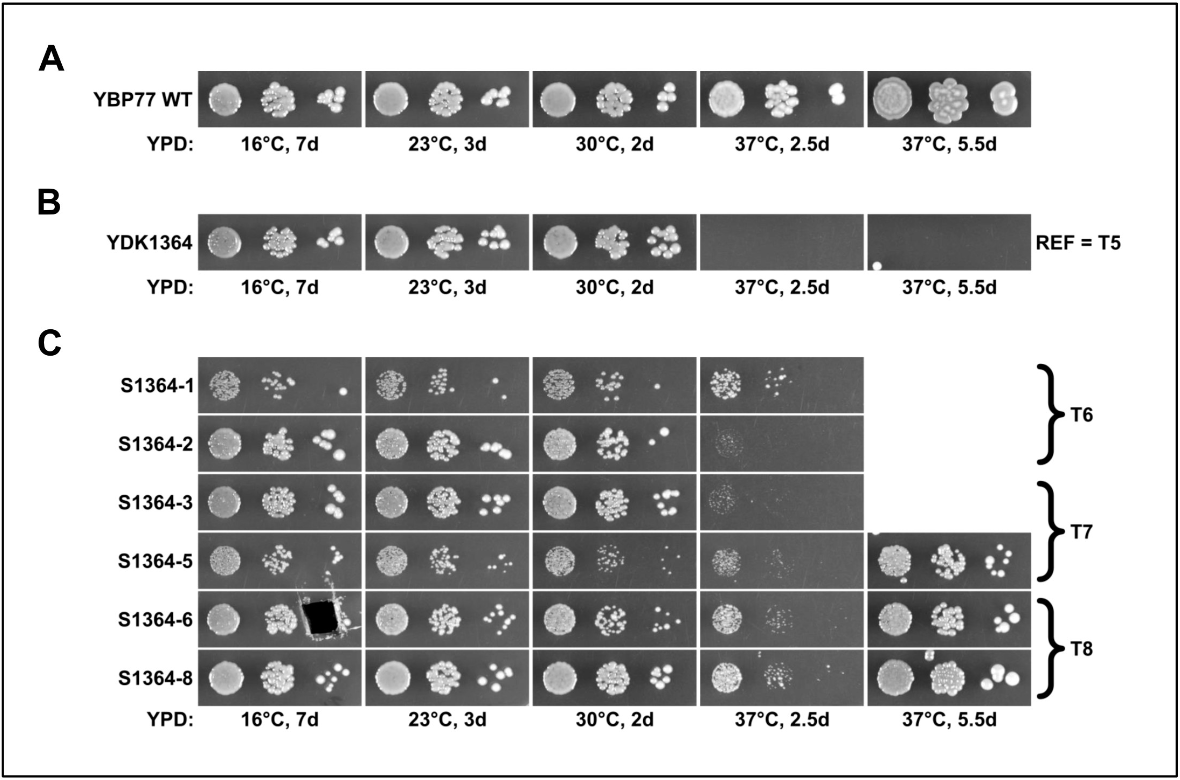
\includegraphics[width=0.7\linewidth]{img/yeastgrowth}
	\caption{\small Growth characteristics of \textit{S.cerevisae} strains cultured in Yeast Extract–Peptone–Dextrose medium (YPD) at different temperatures. Strain names are indicated on the left of the growth assay photographs. \textit{S.cerevisae} cells were plated onto agar plates and were cultured for up to 7 days at increasing temperature starting from 16\degree C to 37\degree C. (A) Wildtype yeast grows well at all tested temperatures. (B) Depicted is the growth behaviour of the $\Delta$TOM1 strain YDK1364, which is highly sensitive to heat. (C) Growth of mutated $\Delta$TOM1 yeast strains derived from YDK1364 that exhibit lower heat susceptibility due to accumulation of mutations that counteract the $\Delta$TOM1 phenotype. Depicted are representative growth assays of the different yeast strains. Adapted from course BC.7107, UNIFR, Benjamin Pillet.}
	\label{fig:yeastgrowth}
\end{figure}


\noindent In this first screening approach, we included only mutations with a Phred-scaled quality score of over 200. Furthermore, we focussed on mutations that interact genetically or physically with TOM1 or genes that encode for ribosomal proteins of the large (RPL) or small (RPS) subunit, because they have observed to accumulate and form detergent-insoluble protein complexes under heat stress. Using our pipeline described in the Methods section, we identified nine mutations that may explain why samples T6, T7, and T8 are less susceptible to high temperatures compared to our reference T5.


\begin{table}[]
	\tiny
	\centering
	\resizebox{\textwidth}{!}{%
		\begin{tabular}{|l|l|l|l|l|}
			\hline 
			\textbf{Sample} & \textbf{Gene Name} & \textbf{Mutation Type} & \textbf{Chromosome} & \textbf{Interactors} \\ \hline
			\textbf{T6} & YGR160W & \begin{tabular}[c]{@{}l@{}}Inframe\\ insertion\end{tabular} & VII & Unknown \\ \hline
			\textbf{T6} & PMT1 & Frameshift & IV & HAS1 \\ \hline
			\textbf{T7} & KRE6 & \begin{tabular}[c]{@{}l@{}}Stop \\ gained\end{tabular} & XVI & \begin{tabular}[c]{@{}l@{}}TOM1,\\   RPL1B, RPL34B\end{tabular} \\ \hline
			\textbf{T7} & KRE9 & Missense & X & \begin{tabular}[c]{@{}l@{}}MRPL17,\\   MRPL25, MRPL38,\\   RPL10, RPL11B,\\   RPL15A, RPL1B,\\   RPL24A, RPL2A,\\   RPL3\end{tabular} \\ \hline
			\textbf{T7} & ISC1 & Missense & V & RPL40B \\ \hline
			\textbf{T7} & FLO9 & \begin{tabular}[c]{@{}l@{}}Inframe \\ insertion\end{tabular} & I & IMG2, YAR1 \\ \hline
			\textbf{T7} & VTC4 & Missense & X & TOM1 (Physical) \\ \hline
			\textbf{T8} & KRE6 & Missense & XVI & \begin{tabular}[c]{@{}l@{}}TOM1, RPL1B, \\   RPL34B\end{tabular} \\ \hline
			\textbf{T8} & ROT1 & Missense & XIII & RPL4B, RPS25A \\ \hline
		\end{tabular}%
	}
\caption{\small Table depicting all heterozygous mutations found in the sample T6 to T8, which might be potential suppressors of the $\Delta$TOM1 phenotype.  Annotation of the mutation type was done by SnpEff. With the exception of VTC4, only genetic interactions are shown. All intergenic and synonymous mutations were excluded from further analysis.}
\label{tab:mutationT68}	
\end{table}

\section*{\large Discussion}

In sample T6, we found two potential high-quality mutation candidates, namely an inframe insertion in \textit{YGR160W} and frameshift mutation in \textit{PMT1}. On closer inspection, we found that \textit{YGR160W} was flagged as a dubious gene, which is unlikely to encode a functional protein, thus in spite of the quality we discarded it from further research. In contrast, \textit{PMT1} codes for an O-mannosyltransferase that is involved in ER quality control among other things\cite{strahl_pmti_1993,goder_protein_2011}. As a result of the enormous global genetic interaction network that has been created by M. Constanzo and colleagues, \textit{PMT1} has been shown to genetically interact with \textit{HAS1}, which codes for an ATP-dependent RNA helicase that is involved in the biogenesis of the 40S and 60S ribosome subunits\cite{costanzo_global_2016,dembowski_has1_2013}.\\ 

\noindent In sample T7, we found an already described\textit{ $\Delta$TOM1} suppressor gene named \textit{KRE6} as well as some putative candidates that might be worth investigating in more depth. We identified a nonsense mutation in the known extragenic suppressor \textit{KRE6} of \textit{$\Delta$TOM1}. The premature stop codon is inserted at nucleotide position 1431 of 2161, which strongly suggests that translation of the \textit{KRE6} transcript results in the formation of a truncated protein. \textit{KRE6} codes for a type II membrane protein involved in the synthesis of $\beta$-(1,6)-glucan, which is an essential constituent of the fungal cell wall\cite{kurita_kre6_2011,roemer_skn1_1993}. In spite of the fact that the function of the KRE6 protein is not directly involved in stress responses, Sasaki and colleagues found that mutation in the \textit{KRE6} gene acts as a weak suppressor of heat sensitivity mediated by \textit{TOM1} deletion\cite{sasaki_extragenic_2000}.\\

\noindent Although the authors were not able to decipher the underlying mechanism responsible for restoring heat tolerance in\textit{ $\Delta$TOM1 S.cerevisae} with mutated \textit{KRE6}, they concluded that the mutation may activate unknown suppressor genes of \textit{$\Delta$TOM1}. According to the Biological General Repository for Interaction Datasets \href{https://thebiogrid.org/}{BioGRID}, \textit{KRE6} has been shown to exhibit genetic interaction with \textit{TOM1} itself as well as multiple genes coding for mitochondrial and cytoplasmic ribosomal proteins of the large subunit (Table \ref{tab:mutationT68}). Moreover, we found a missense mutation in gene \textit{KRE9}, which is also involved in the synthesis of $\beta$-(1,6)-glucan like KRE6 protein. The deletion of \textit{KRE9}  has long been known to have a deleterious effect on the growth of \textit{S.cerevisae} by altering the composition of its cell wall\cite{brown_yeast_1993}. Similar to \textit{KRE6}, \textit{KRE9} also interacts with several genes coding for the small and large subunits of ribosomes (Table \ref{tab:mutationT68}). It is also conceivable that \textit{KRE9} mutation alone or in combination with the mutation in \textit{KRE6} has an impact on the transcription of ribosomal genes and thus may passively counteract the stress response associated with the accumulation of protein related to \textit{$\Delta$TOM1}. Another gene related to ribosome biogenesis was also found to be mutated in sample T7, namely \textit{ISC1}, which has been reported to interact genetically with \textit{RPL40B}\cite{hoppins_mitochondrial-focused_2011}. While the protein ISC1 is not directly linked to the regulation of ribosome biosynthesis, RPL40B is involved in the maturation of the 60S ribosomal subunit\cite{fernandez-pevida_yeast_2012}. Interestingly, the null mutation of \textit{ISC1} has been associated with heat sensitivity, which implies that the mutation observed in sample T7 does not yield a non-functional protein. Therefore, we concluded that the mutation in \textit{ISC1} is most likely not responsible for counteracting the heat-sensitive phenotype resulting from the deletion of \textit{TOM1}. Last but not least, we also identified a mutation in a direct physical interactor of the TOM1 protein in sample T7 named VTC4, which is a component of the vacuolar transporter chaperone (VTC) complex\cite{muller_role_2003}. Unfortunately, the nature of the interaction between VTC4 and TOM1 is not described and thus it is not possible to evaluate whether a mutation in this gene has an impact on the \textit{$\Delta$TOM1} phenotype.\\
 
\noindent In T8, we observed a missense mutation in \textit{KRE6}. In addition, we discovered another missense mutation in a gene named \textit{ROT1}, which codes for a chaperone involved in protein folding\cite{takeuchi_saccharomyces_2008}. Similar to the other gene candidates, \textit{ROT1} also interacts genetically with ribosomal genes, namely \textit{RPL4B} and \textit{RPS25A}.\\
 
\noindent Interestingly, most of the mutations we found in samples T6, T7, and T8 were indirectly linked to genes coding for ribosomal proteins. These findings are of particular interest since deletion of \textit{TOM1} has been associated with an accumulation of ribosomal proteins. Under normal conditions, the E3 ubiquitin ligase TOM1 rapidly removes excess of ribosomal proteins via proteasomal degradation\cite{sung_conserved_2016}. In conclusion, we found one known as well as seven potential new suppressors of \textit{$\Delta$TOM1}. The known suppressor \textit{KRE6}, has been found to be mutated in T7 and T8. Due to the heterozygosity of the mutation, we conclude that \textit{KRE6} may explain the partially restored capability of \textit{S.cerevisae} to grow at 37\degree C in one of the two strains found in each sample. However, it is important to note that while the mutation in T7 introduces an additional stop codon, the spontaneous mutation in T8 only changed one amino acid and consequently affects the function of the protein to a lesser extent (Table \ref{tab:mutationT68})\cite{sasaki_extragenic_2000}. Since most of the mutated genes found in our samples were associated with biogenesis or regulation of ribosomes, it would be interesting to investigate whether these mutations suppress the accumulation of ribosomal proteins in the absence of \textit{TOM1}. Taken together, our data provide the basis for further investigations aimed at clarifying whether accumulation of ribosomal proteins may be causative of the heat sensitivity of yeast lacking \textit{TOM1}.
 
 
 
 
 
 









%%%%%%%%%%%%%%%%%%%%%%%%%%%%%%%%%%%%%%%%%%%%%%%%%%%%%%%%%%%%
%%%%%%%%%%%%%%%%%%%%%%%%%%%%%%%%%%%%%%%%%%%%%%%%%%%%%%%%%%%%
%%%%%%%%%%%%%%%%%%%%%%%%%%%%%%%%%%%%%%%%%%%%%%%%%%%%%%%%%%%%
\newpage
\part*{\Large Identification of \textit{gai} phenotype revertant mutations in \textit{Arabidopsis thaliana}}

\href{mailto:thibault.schowing@unifr.ch}{Thibault Schowing}, \href{mailto:lio_roh@students.unibe.ch}{Lionel Rohner},
\href{mailto:alain.rohrbasser.unifr.ch}{Alain Rohrbasser},
\href{mailto:rares.cristea@unifr.ch}{Rares Cristea}\\

\section*{\large Introduction}
Gibberellic Acid (GA) is a growth factor that influences essentially the stem elongation and other plant developmental processes\cite{hooley_gibberellins:_nodate}. The study of plants deficient in the biosynthesis of this hormone has been essential to agriculture. Selective breeding of these mutant plants  was one of the key factors leading to the green revolution since 1960, thus increasing the yield of the crops. Hence, the study of plant’s response to GA is still essential for many agricultural applications\cite{ordonio_new_2017}. Gibberellic-Acid Insensitive (\textit{GAI}) is a gene in \textit{Arabidopsis thaliana} (\textit{A. thaliana}) in chromosome 1 which is involved in the regulation of plant growth. More precisely, it modulates plant growth by decreasing the responsiveness to GA\cite{peng_arabidopsis_1997}. (\textit{GAI}) encodes for a protein containing a DELLA domain, which interacts with a receptor bound GA, and a functional GRAS-domain. When GA binds to its receptor GID1, they form a complex with DELLA and recruit an utiquitin ligase named SCFSLY1. DELLA is then ubiquinated and degraded in the proteasome (Figure \ref{fig:gaspypathway})\cite{hauvermale_gibberellin_2012}. The CS63 strain contains a 51bp deletion in the DELLA-domain of \textit{GAI}. The deletion acts as a gain-of-function mutation in DELLA, thus resulting in a dwarf phenotype due to its reduced sensitivity to GA-signaling\cite{peng_arabidopsis_1997,lee_gibberellin_2002}.\\


\noindent SPINDLY (\textit{SPY}) is a gene coding for a peptide sequence that is thought to interact and activate DELLA, and thus negatively regulates GA signaling pathway\cite{zentella_arabidopsis_2017}. Three independent recessive mutations at the \textit{SPY} locus of \textit{A. thaliana} gives resistance to the paclobutrazol inhibitor molecule in the GA biosynthesis pathways. This confers to the spy mutants an other phenotype also observed when wild-type \textit{A. thaliana} plants are constantly treated with GA. The \textit{spy-1} allele\footnote{Mutant alleles are written in lower-case.} is partially epistatic to the loss-of-function mutation of \textit{gai}, that causes GA defect. Furthermore, the \textit{spy-1} mutation can together suppress the repercussion of the loss-of-function mutation of \textit{gai} and paclobutrazol therapy, which inhibit diverse steps in the GA biosynthesis pathway\cite{lee_gibberellin_2002, jacobsen_mutations_nodate}.\\

%http://genesdev.cshlp.org/content/16/5/646


\noindent The aim of this project was to screen two mutant strains of \textit{A. thaliana} that were generated by random $\gamma$-ray mutagenesis of CS63 for mutations in gene \textit{GAI} and \textit{SPY}. As opposed to C63, Gar12 and Gar13 exhibit normal growth and we hypothesized that random mutation in \textit{GAI} and/or \textit{SPY} may be causative for their phenotypic reversion.\\


\begin{figure}[h]
	\centering
	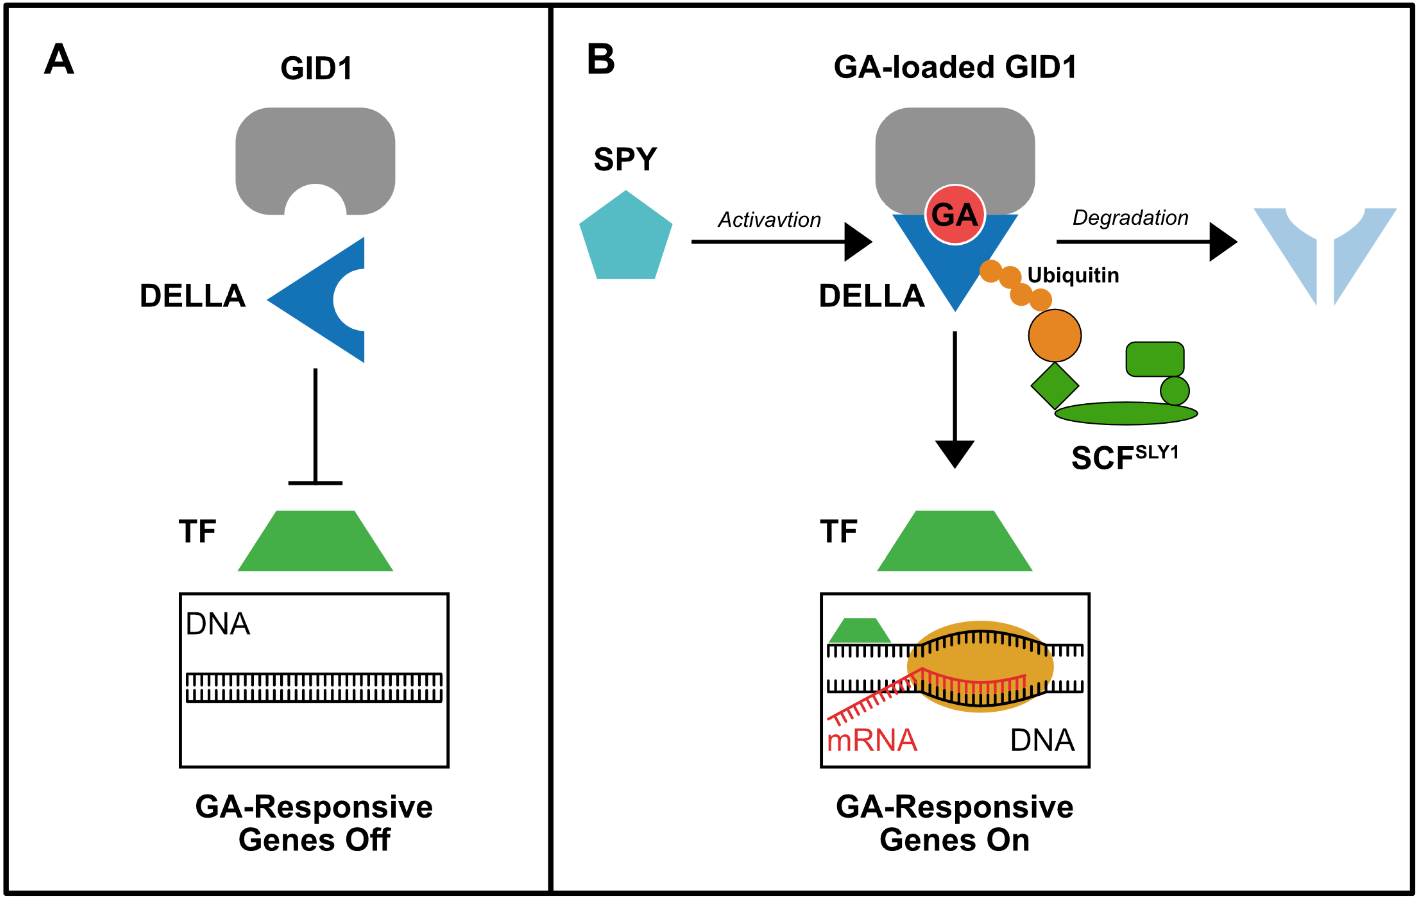
\includegraphics[width=0.6\linewidth]{img/GAI_SPY_Introcut}
	\caption[GAI and SPY pathways]{ (A) In the abscence of GA, DELLA is not able to interact with GID1. Free DELLA proteins sequester transcription factors (TF) that activate GA-responsive genes, thus preventing growth. (B) In the presence of GA, GID1 and GA form a ligand-receptor complex that favors binding of DELLA. Once bound to GA-loaded GID1, DELLA is ubiquitinated by SCF$^{SLY1}$ and eventually degraded, thus promoting growth. Recent findings suggest that SPY can counteract the activation of GA-responsive genes by activating DELLA by fucosylation. Adapted from  Adapted from \cite{hauvermale_gibberellin_2012}.}
	\label{fig:gaspypathway}
\end{figure}




\section*{\large Methods} 

\paragraph{Trimming, Read Group Informations, Aligning and MarkDuplicates} After the quality control check with \textit{FastQC}\cite{andrews2012}, \textit{Trimmomatic}\cite{bolger_trimmomatic:_2014} was used to filter out bad quality reads. Only the ones with a minimal length of 140 and an average quality of 15 were kept. The \textit{bwa} (Burrows-Wheeler Aligner) tool was then used to index the reference genome and to align all the reads against this reference while adding the Read Group Information at the same time. The resulting SAM files were then sorted and converted into BAM files through  \href{https://software.broadinstitute.org/gatk/documentation/tooldocs/4.0.8.0/picard_sam_SortSam.php}{SortSam} (\href{https://broadinstitute.github.io/picard/}{Picard}) and the duplicate reads were marked using  \href{https://software.broadinstitute.org/gatk/documentation/tooldocs/4.0.4.0/picard_sam_markduplicates_MarkDuplicates.php}{MarkDuplicates} (\href{https://broadinstitute.github.io/picard/}{Picard}). This step, takes a sorted BAM file and add information about reads that might come from the same DNA fragment, in order to avoid counting the information given by one fragment more than one time. 

\paragraph{Haplotype Caller and Base Quality Score Recalibration} Since the genome of the \textit{A. thaliana} is diploid, the  \href{https://software.broadinstitute.org/gatk/documentation/tooldocs/3.8-0/org_broadinstitute_gatk_tools_walkers_haplotypecaller_HaplotypeCaller.php}{Haplotype Caller} (\href{https://software.broadinstitute.org/gatk/}{GATK4})was used to have a first variant call. The VCF file was then split in two, one containing only the INDELs information, and one containing the SNPs, with  \href{https://software.broadinstitute.org/gatk/documentation/tooldocs/3.8-0/org_broadinstitute_gatk_tools_walkers_variantutils_SelectVariants.php}{SelectVariants} (\href{https://software.broadinstitute.org/gatk/}{GATK4}) because the filtration methods differ. Then the new VCF files were filtered to get rid of all the false variants, through  \href{https://software.broadinstitute.org/gatk/documentation/tooldocs/3.8-0/org_broadinstitute_gatk_tools_walkers_filters_VariantFiltration.php}{VariantFiltration} (\href{https://software.broadinstitute.org/gatk/}{GATK4}), using different parameters for INDELs and for SNPs. Then the \href{https://gatkforums.broadinstitute.org/gatk/discussion/44/base-quality-score-recalibration-bqsr}{BQSR}, a data pre-processing step that detects systematic errors made by the sequencer when it estimates the quality score of each base call, was performed in two iteration to recalibrate the original bam files. A final variant call was made to generate a single vcf file containing both SNPs and INDELs. 

\paragraph{Annotation}
For the annotation step, \href{http://snpeff.sourceforge.net/}{SnpEff} was used in order to annotate the VCF file, to get rid of all the synonymous and intergenic variants and also to keep only the variants that are found in less than 2 strains. The analysis was further done by using \href{http://www.phenosystems.com/www/index.php/products/gensearchngs}{GeneSearch} (\href{http://www.phenosystems.com/www/}{GeneSearch}), and since the whole BAM files were too big to handle, a shortened version of the BAM files, containing only the information about the \textit{GAI} gene on the first chromosome, and the \textit{SPY} gene on the third chromosome was used.


\section*{\large Results}

We found that Gar13 had the original mutation in the DELLA-domain of the \textit{GAI} gene, whereas Gar12 had a deletion at the same location, but affected 52 nucleotides instead of 51 like in the original deletion found in C63 (Table \ref{tab:resultATH}). Furthermore, we found one additional frameshift deletion in the functional GRAS-domain of strain Gar13. In \textit{SPY} only one single missense mutation that was present in both strains was found. 


% Please add the following required packages to your document preamble:
% \usepackage{graphicx}
\begin{table}[h]
	\centering
	
		\begin{tabular}{|l|l|l|l|l|}
			\hline
			\textbf{Strains} & \textbf{Gene} & \textbf{Chromosome} & \textbf{Position} & \textbf{Mutation type} \\ \hline
			Gar12 & \textit{GAI} & I & 5'149’424 & 3bp inframe deletion (ATC) \\ \hline
			Gar12 & \textit{GAI} & I & 5'149’496 & 52bp frameshift Deletion \\ \hline
			Gar12 & \textit{SPY} & III & 3'637’438 & Missense mutation: T\textgreater{}C \\ \hline
			Gar13 & \textit{GAI} & I & 5'149’424 & 3bp inframe Deletion (ATC) \\ \hline
			Gar13 & \textit{GAI} & I & 5'149’495 & 51bp inframe Deletion (DELLA) \\ \hline
			Gar13 & \textit{GAI} & I & 5'149’624 & 1bp frameshift deletion (G) \\ \hline
			Gar13 & \textit{SPY} & III & 3'637’438 & Missense mutation: T\textgreater{}C \\ \hline
		\end{tabular}
	\caption{Table showing all non-synonymous mutations found in \textit{A. thaliana} strains Gar12 and Gar13.}
	\label{tab:resultATH}
\end{table}

\paragraph{Discussion}

Due to the additional nucleotide affected by the large deletion in Gar12, the deletion leads to a frameshift that affects all codons upstream of the DELLA-domain and thus substantially affects the structural integrity of DELLA. This means that although the \textit{GAI} gene exhibits a gain-of-function mutation, which renders the protein resistant to proteasomal degradation, the deletion changes a substantial number of amino acids in the functional GRAS-domain. Therefore the repressive effect of DELLA is subverted and the plant is able to thrive (Figure \ref{fig:delladomains}).\\


\noindent In the Gar13 strain, the gain-of-function deletion of 51bp of the DELLA region is present, meaning that the phenotypic reversion is not given by the presence of the DELLA domain, but rather by another mutation in the functional domain. We assume that the only mutation that could be able to abrogate the gain-of-function mutation in DELLA is a single nucleotide, which induces a frameshift in the reading frame and thus probably affects the functional GRAS-domain (Table \ref{tab:resultATH} and Figure \ref{fig:delladomains}). Similar to Gar12, this strain is able to grow normally, due to inactivation of the DELLA protein (Figure \ref{fig:delladomains}).


\begin{figure}[H]
	\centering
	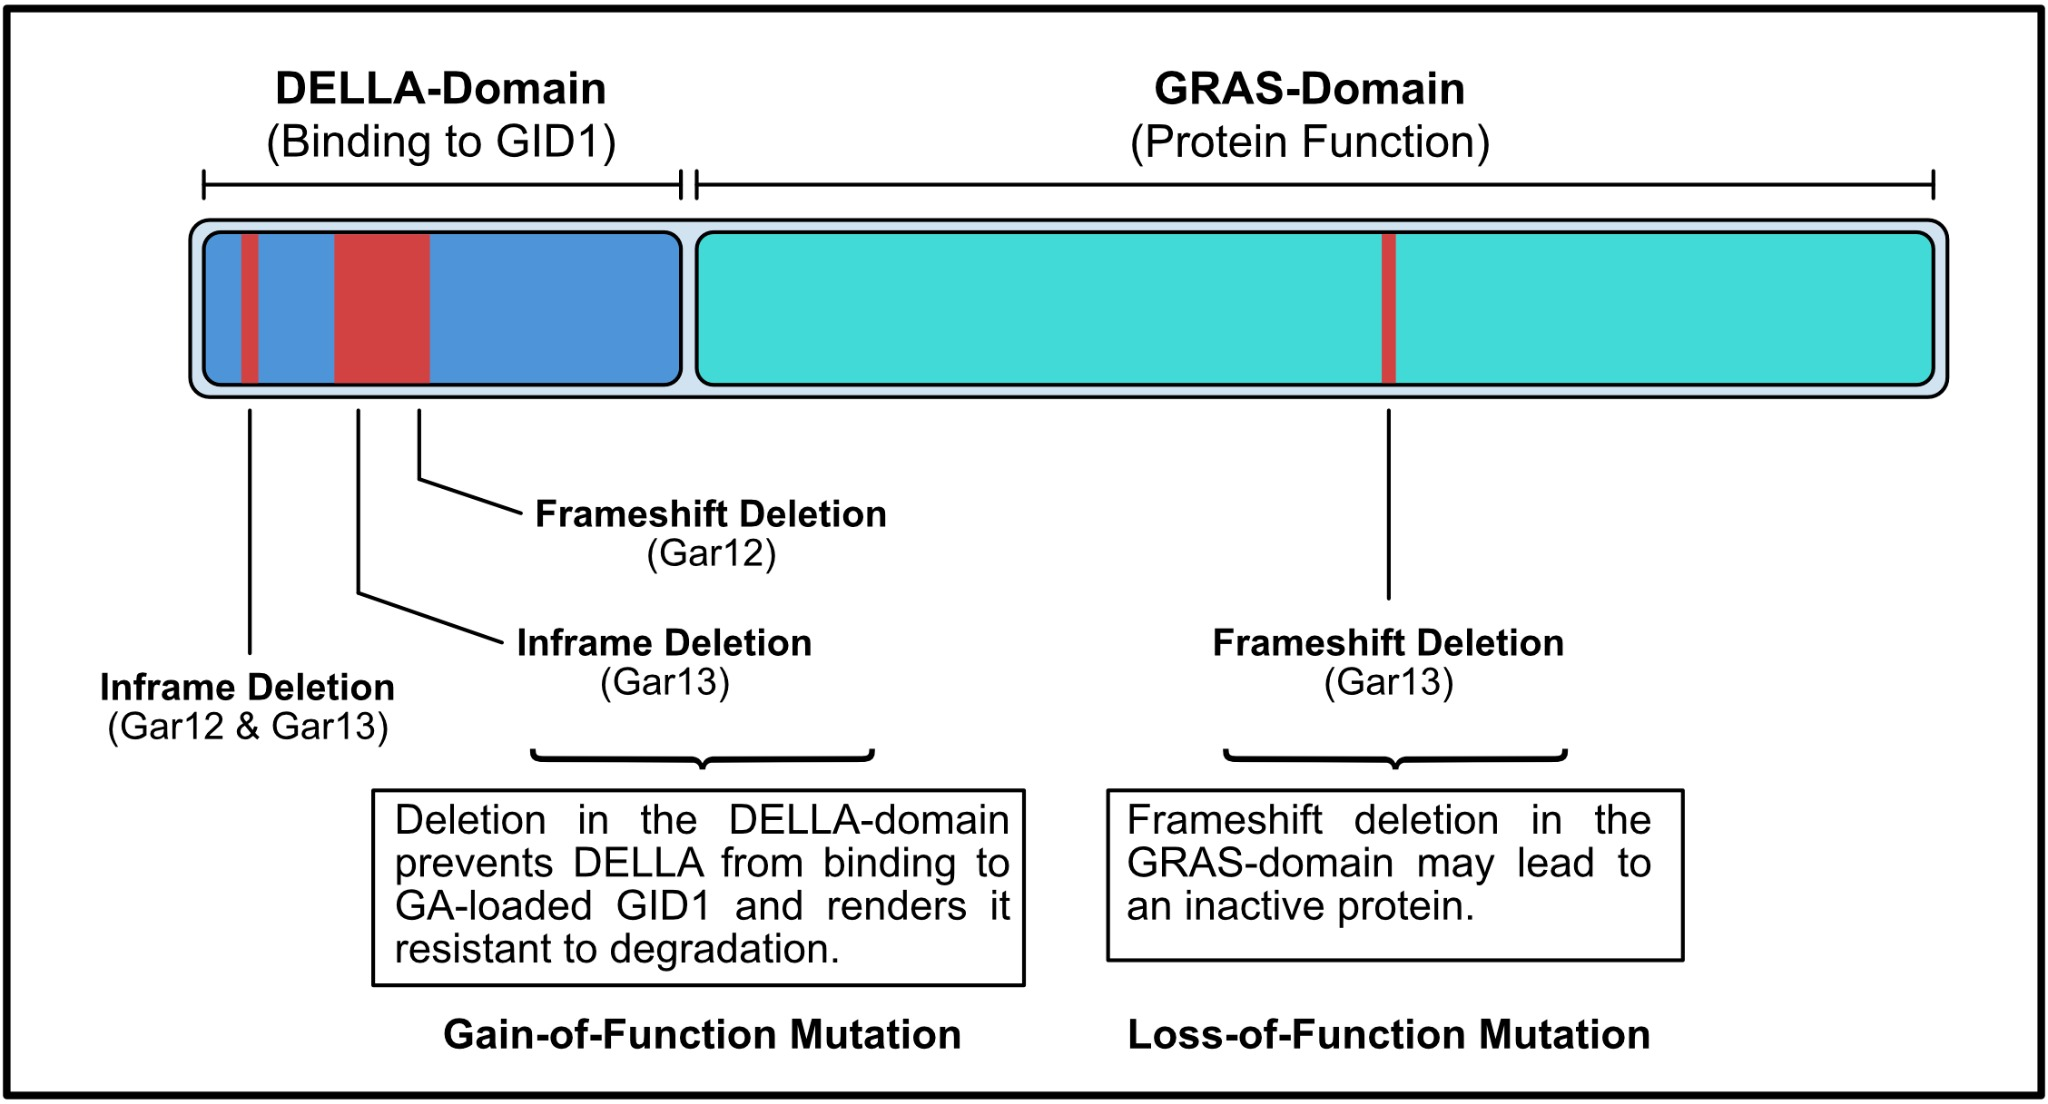
\includegraphics[width=0.7\linewidth]{img/DELLAdomains}
	\caption{Illustrative summary of the project. The DELLA protein is shown with its main domains. Regions highlighted in red represent deletions that were found in Gar12 and/or Gar13.}
	\label{fig:delladomains}
\end{figure}



\noindent The other 3bp deletion, which was discovered downstream of the primary deletion, is probably redundant as the 51bp deletion prevents DELLA from binding to GA-loaded GID1 regardless of other mutations. Furthermore, this variant is found in both Gar12 and Gar13, which suggests that the mutation did not arise from random mutagenesis, but was probably already present in C63. Since loss-of-function mutations in \textit{SPY} are known to suppress gain-of-function mutations in \textit{GAI}, we also searched for potential non-synonymous mutations in \textit{SPY}. However, in both strains, we only found one missense variant in the \textit{SPY} gene, changing a valine to alanine in the amino acid chain. This mutation is unlikely to have an impact on the function of SPY since the amino acid substitution (V to A) is a conservative replacement with a low impact on biochemical properties. Moreover, similar to the 3bp inframe deletion in \textit{GAI}, this mutation was also found in both Gar12 and Gar13 and was therefore presumably present in the original plant C63. Taken together, Gar12 and Gar13 do not exhibit the dwarf phenotype due to mutations in the functional GRAS-domain of GAI rather than loss-of-function mutations in \textit{SPY}(Figure \ref{fig:delladomains}).





%%%%%%%%%%%%%%%%%%%%%%%%%%%%%%%%%%%%%%%%%%%%%%%%%%%%%%%%%
%%%%%%%%%%%%%%%%%%%%%%%%%%%%%%%%%%%%%%%%%%%%%%%%%%%%%%%%%
%%%%%%%%%%%%%%%%%%%%%%%%%%%%%%%%%%%%%%%%%%%%%%%%%%%%%%%%%
%%%%%%%%%%%%%%%%%%%%%%%%%%%%%%%%%%%%%%%%%%%%%%%%%%%%%%%%%
\newpage
\part*{\Large \textit{Lactobacillus Heleveticus} Genome De Novo Assembly}

\href{mailto:thibault.schowing@unifr.ch}{Thibault Schowing}, \href{mailto:lio_roh@students.unibe.ch}{Lionel Rohner},
\href{mailto:alain.rohrbasser.unifr.ch}{Alain Rohrbasser},
\href{mailto:rares.cristea@unifr.ch}{Rares Cristea}\\

\section*{\large Introduction}

The diverse bacteria involved in cheese production are essential for the texture and taste development but also, during the ripening process, the microbial changes help to kill pathogens and reduce spoilage microorganisms. \textit{Lactobacillus helveticus} (\textit{L. helveticus})is a thermophilic lactic acid bacterium (LAB) used in the dairy industry as a starter as well as an adjunct culture for cheese manufacture\cite{kongo_lactic_2013}. During cheese ripening LAB undergo autolysis, which is a lytic event of the bacterial cell caused by its own intracellular enzymes, named autolysins or peptidoglycan hydrolases (PGHs)\cite{delcour_biosynthesis_1999}. Autolysis of the bacteria leads to the release of these enzymes, which have the ability to digest the cell wall peptidoglycan of surrounding Gram+ bacteria and thus reduce microbial spoilage of the cheese\cite{jebava_nine_2011}. The genomic plasticity of \textit{L. helveticus} leads to a high variation in PGHs activity from one strain to another. In a previous study\cite{jebava_nine_2011}, nine genes coding PGHs were annotated and the activity of a PGH with an estimated size of 30kDa was tested by zymography in nine strains of \textit{L. helveticus} of which six were sequenced (Figure \ref{fig:zymography}). Two phenotypes were shown: phenotype A exhibits PGH activity (strains \textbf{FAM8102c1c1}, \textbf{FAM23285} and \textbf{FAM19191}) and phenotype B does not (strains \textbf{FAM22016}, \textbf{FAM1450} and \textbf{FAM1213}).\\

%\noindent The aim of this work was to detect potential genomic differences involved in the two different phenotypes by sequencing, assembling and compare the genome of the six strains using a previously annotated reference genome of \textit{Lactobacillus helveticus} (\href{https://www.ncbi.nlm.nih.gov/genome/?term=NC_010080}{NC\_010080}). A potential candidate present only in the strains expressing a PGHs activity suggests that it might have been acquired by a viral insertion. 

\noindent The aim of this project was to perform a de novo assembly and annotation of the genomes of the above mentioned \textit{L. helveticus} strains, in order to detect potential genomic differences between phenotype A and phenotype B.

\section*{\large Methods}

\paragraph{Sequencing and genome assembly}
The six \textit{L. helveticus} strains \textbf{FAM8102c1c1}, \textbf{FAM23285}, \textbf{FAM19191}, \textbf{FAM22076}, \textbf{FAM1450}, \textbf{FAM1213}  were sequenced by Illumina sequencing (Illumina, SanDiego, CA, USA). The following tasks were performed using the cluster provided by the University of Bern.  \textit{FastQC}\cite{andrews2012} was used to check the quality of the reads and \textit{Trimmomatic}\cite{bolger_trimmomatic:_2014} to filter out bad quality reads. Only the ones with a minimal length of 100 and an average quality of 8 were kept. \textit{\href{http://www.gigasciencejournal.com/content/1/1/18/}{SOAPdenovo}\footnote{Cited as requested by the authors but the content is not accessible.}} as well as \textit{SPAdes}\cite{hutchison_assembling_2013} were used to perform the genome assembly with the reads of each strains. For \textit{SOAPdenovo} the k-mer sizes were set to 95, 85, 75 and 65. For \textit{SPAdes} k-mere sizes were set to 21, 33, 55, 77 and 99 (default values). The four assemblies of SOAPdenovo and the assembly of \textit{SPAdes} were compared using Abyss\cite{simpson_abyss:_2009} with a maximum number of contigs set to 1000. The best genome assemblies with the bigger N50 and an approximate genome size of 20Mbp (Genome size of \textit{L. helveticus}) were chosen\footnote{Due to the temporary unavailability of the cluster, this operation has been performed by L. Falquet and the results were provided to the students afterwards.}.






\paragraph{Genome annotation and pan-genome analysis}
We used the \textit{PROKKA} pipeline\cite{seemann_prokka:_2014} to annotate the genome of the six best assemblies and the reference genome of \textit{L. helveticus} \href{https://www.ncbi.nlm.nih.gov/genome/?term=NC_010080}{NC\_010080}. \textit{PROKKA} is an automated pipeline that annotates prokaryotic genomes. It locates open reading frames and RNA regions on contigs and translates it to protein sequences, searching for protein homologues in public databases. The resulting standards \href{https://www.ensembl.org/info/website/upload/gff.html}{.gff} files containing the annotated genome for each strain were then used by \textit{Roary}\cite{page_roary:_2015} to generate a pan-genome of the six strains. The result was then visualized with \textit{Phandango}\cite{hadfield_phandango:_2018} allowing visualisation of phylogenetic tree, associated metadata, and genomic information.


\paragraph{Extraction of the genes for each phenotypes} Grep was used on the files generated by \textit{Roary} to extract the nine PHG's \cite{jebava_nine_2011} labelled "Lhv\_" with \textit{PROKKA} (Appendix \ref{tab:resultCommonLhv}). The set of genes found in strains expressing phenotype A was compared to the set of gene showing phenotype B. In Table \ref{tab:resultPGHexpr} we have the two PGHs present only in the three strains expressing the PGHs activity. 


\begin{figure}
	\centering
	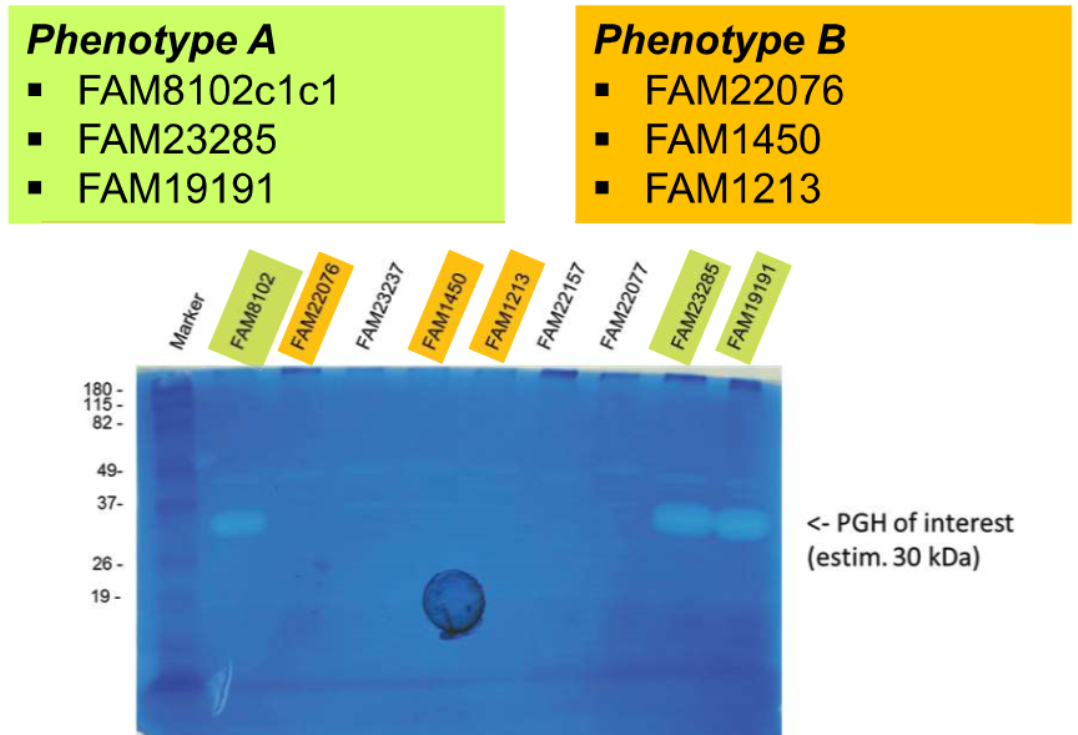
\includegraphics[width=0.7\linewidth]{img/zymography}
	\caption[The two phenotypes expressed by the six strains]{Result of a zymogram of the different \textit{L. helveticus} strains of interest. The zymogram reveals that strains with phenotype A (green) express an active PGH with a size of about 30 kDa. In contrast, strains with phenotype B (yellow) appear to have lost the activity of the enzyme or possibly do not express it at all.}
	\label{fig:zymography}
\end{figure}


\section*{\large Results}


\begin{table}[htbp]
	\centering
	\begin{tabularx}{\linewidth}{|X|X|X|X|X|X|}
		\hline
		\textbf{Gene} & \textbf{Annotation} & \textbf{Avg group size [nt]} & \textbf{FAM19191\_ 1K} & \textbf{FAM23285\_ 1K} & \textbf{FAM8102\_ 1K}\\
		 \hline
		%group\_1899 & Lhv\_2053 Lysin (L.crispatus) pseudogene in L.helveticus & 830/ 30 kDa & FAM19191\_ 1K\_00615 & FAM23285\_ 1K\_00607 & FAM8102\_ 1K\_00746 \\
		%\hline
		group\_2348 & Lhv\_2053 Lysin (L.crispatus) pseudogene in L.helveticus & 1121 bp  \newline     41 kDa & FAM19191\_ 1K\_00069 & FAM23285\_ 1K\_00060 & FAM8102\_ 1K\_00069 \\
		\hline
		group\_2372 & Lhv\_2053 Lysin (L.crispatus) pseudogene in L.helveticus & 893 bp    \newline    33 kDa & FAM19191\_ 1K\_00397 & FAM23285\_ 1K\_00499 & FAM8102\_ 1K\_00565 \\
		\hline	
	\end{tabularx}
	\caption{Genes present only in the three strains with a PGH activity. To convert nt to kDa the Bioline DNA to Protein \href{https://www.bioline.com/us/media/calculator/01_06.html}{Converter} was used.}
	\label{tab:resultPGHexpr}
\end{table}

\noindent According to the zymography (Figure \ref{fig:zymography}), the PGH involved is approximately 30kDa thus matches with group 2372. Looking at the alignment of the amino acid sequences in the output files,
%(Figure \ref{fig:alignmentgrp2372}) 
we saw that the sequences are identical, suggesting that it is conserved among the three strains. \\


\paragraph{Discussion} We can see that PGHs are present in all strains (Appendix \ref{tab:resultCommonLhv}), therefore the phenotype is not due to an absence of PGH (Figure \ref{fig:zymography}). With \textit{Roary} we identified a \textit{PGH} pseudogene that was present in the three strains exhibiting phenotype A with a matching molecular weight. The fact that it is labelled as \textit{pseudogene} can mean that it might have lost part of its functionality and further investigation would be needed to assess the activity of the protein.\\

\noindent Using BLASTp\cite{altschul_gapped_1997} with default parameters, the protein was searched to be a particular lysin (\href{https://www.ncbi.nlm.nih.gov/protein/1325986555}{WP\_101853908.1}) encoded by the pneumococcal bacteriophage Cp-1\cite{martin_pneumococcal_1998}. To look further into this sequence, we used PHASTER \cite{arndt_phaster:_2016}, the PHAge Search Tool - Enhanced Release, which helps identifying and annotating prophage sequences within bacterial genomes and plasmids. The research was made only for \textbf{FAM19191}, as the sequence is identical in the three strains. The result indicating a highly conserved muramidase sequence (Figure \ref{fig:phasterresultmuramidase}A) confirms that the PGH oroginates from a phage. The locus is also shown (Figure \ref{fig:phasterresultmuramidase}B). 

\begin{figure}[H]
	\centering
	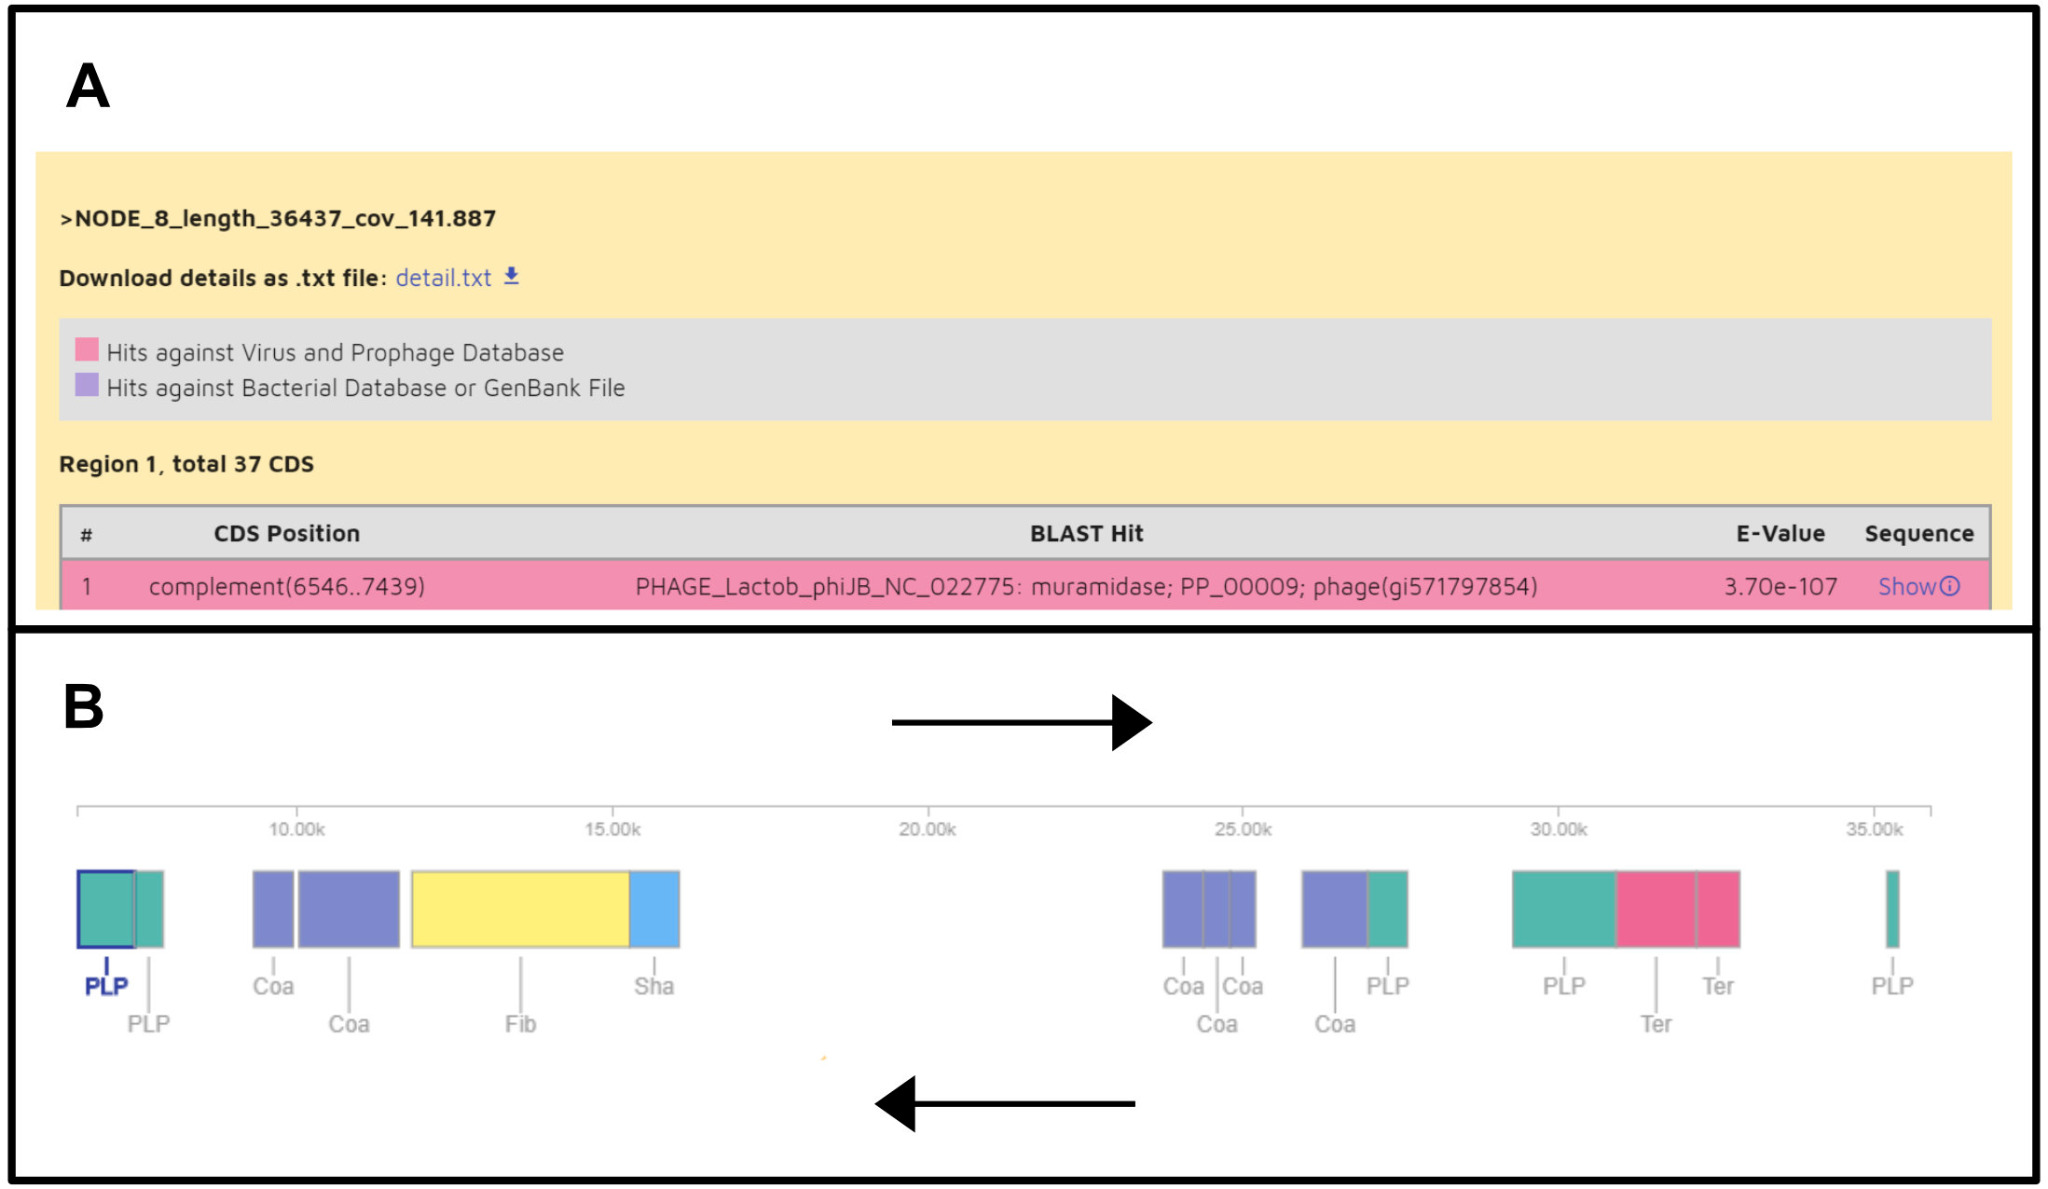
\includegraphics[width=0.7\linewidth]{img/fasterfasterfucker}
	\caption{(A)Partial result with the assembly of \textbf{FAM19191} run in PHASTER. (B)Node 8 of \textbf{FAM19191} assembly showing annotated locus. The highlited locus represents the phage-derived muramidase.}
	\label{fig:phasterresultmuramidase}
\end{figure}





\noindent Many gene sequences of other PGHs, pseudogenes and hypothetical proteins were found in some or all of the six different strains (Appendix \ref{tab:resultCommonLhv}). It would be interesting to pursue further analysis of the transcription and expression of these sequences, to further unravel the differences between the strains. The increased production of PGHs can be of major importance, especially in cheese ripening. The PGHs present in all strains and the ones present only in a small subset are most certainly located on the core-genome and the pan-genome, respectively. However, some of them might be absent only in one or two of all the strains and might be labelled as part of the "soft-core" or the "shell" genome \cite{kaas_estimating_2012,inglin_clustering_2018} as we can see in the summary statistics produced by \textit{Roary}.

\newpage


\begin{multicols}{2}
	\bibliography{mybib}{}
	\bibliographystyle{ieeetr}
\end{multicols}	

\appendix
\setcounter{table}{0}  


\part*{\Large Appendix}
\begin{landscape}
	\begin{table}[h]
		\begin{tabularx}{\linewidth}{|l|l|X|X|X|X|X|X|}\hline
			Gene & Annotation & FAM1213 1K & FAM1450 1K & FAM19191 1K & FAM22076 1K & FAM23285 1K & FAM8102 1K \\\hline
			
			group\_1103 & \begin{tabular}[c]{@{}l@{}}Lhv\_0549 \\N-acetylmuramidase \end{tabular} & FAM1213\_ 1K\_01187 & FAM1450\_ 1K\_00785 & FAM19191\_ 1K\_01147 & FAM22076\_ 1K\_00934 & FAM23285\_ 1K\_01072 & FAM8102\_ 1K\_01185 \\\hline
			
			group\_1218 & \begin{tabular}[c]{@{}l@{}}Lhv\_1433 Lysin \end{tabular} & FAM1213\_ 1K\_01833 & FAM1450\_ 1K\_00044 & FAM19191\_ 1K\_01884 & FAM22076\_ 1K\_01582 & FAM23285\_ 1K\_01903 & FAM8102\_ 1K\_01986 \\\hline
			
			group\_3457 & \begin{tabular}[c]{@{}l@{}}Lhv\_0649 Lysozyme \end{tabular} & FAM1213\_ 1K\_00895 & FAM1450\_ 1K\_00838 & FAM19191\_ 1K\_01232 & FAM22076\_ 1K\_00917 & FAM23285\_ 1K\_01191 & FAM8102\_ 1K\_01268 \\\hline
			
			group\_852 & \begin{tabular}[c]{@{}l@{}}Lhv\_1295 \\Enterolysin M23 \\family peptidase \end{tabular} & FAM1213\_ 1K\_00043 & FAM1450\_ 1K\_01113 & FAM19191\_ 1K\_00150 & FAM22076\_ 1K\_00164 & FAM23285\_ 1K\_00217 & FAM8102\_ 1K\_00225 \\\hline
			
			group\_862 & \begin{tabular}[c]{@{}l@{}}Lhv\_1059 \\LysM \\peptidoglycan\\binding\\ domain-containing \\protein\end{tabular} & FAM1213\_ 1K\_00147 & FAM1450\_ 1K\_00238 & FAM19191\_ 1K\_00248 & FAM22076\_ 1K\_00274 & FAM23285\_ 1K\_00308 & FAM8102\_ 1K\_00381 \\\hline
			
			group\_993 & \begin{tabular}[c]{@{}l@{}}Lhv\_1433 Lysin \end{tabular} & FAM1213\_ 1K\_00691 & FAM1450\_ 1K\_01203 & FAM19191\_ 1K\_01800 & FAM22076\_ 1K\_00088 & FAM23285\_ 1K\_01748 & FAM8102\_ 1K\_01891 \\\hline
			
			group\_995 & \begin{tabular}[c]{@{}l@{}}Lhv\_0191 \\Amidase \end{tabular} & FAM1213\_ 1K\_00700 & FAM1450\_ 1K\_00303 & FAM19191\_ 1K\_00506 & FAM22076\_ 1K\_00064 & FAM23285\_ 1K\_00566 & FAM8102\_ 1K\_00638 \\\hline
			
			group\_1862 & \begin{tabular}[c]{@{}l@{}}Lhv\_2053 Lysin \\(L.crispatus) \\pseudogene\\   in L.helveticus\end{tabular} &  & FAM1450\_ 1K\_00045 & FAM19191\_ 1K\_01885 & FAM22076\_ 1K\_01583 & FAM23285\_ 1K\_01904 & FAM8102\_ 1K\_01987 \\\hline
			
			group\_1899 & \begin{tabular}[c]{@{}l@{}}Lhv\_2053 Lysin \\(L.crispatus) \\pseudogene\\   in L.helveticus\end{tabular} &  & FAM1450\_ 1K\_00267 & FAM19191\_ 1K\_00615 & FAM22076\_ 1K\_00716 & FAM23285\_ 1K\_00607 & FAM8102\_ 1K\_00746 \\\hline
			
			group\_1344 & \begin{tabular}[c]{@{}l@{}}Lhv\_1307 \\Enterolysin M23 \\family peptidase \end{tabular} &  &  & FAM19191\_ 1K\_00162 & FAM22076\_ 1K\_00152 & FAM23285\_ 1K\_00229 & FAM8102\_ 1K\_00237 \\\hline
			
			group\_1345 & \begin{tabular}[c]{@{}l@{}}Lhv\_0190 \\N-acetylmuramidase \end{tabular} &  &  & FAM19191\_ 1K\_00507 & FAM22076\_ 1K\_00063 & FAM23285\_ 1K\_00565 & FAM8102\_ 1K\_00639 \\
			\hline
		\end{tabularx}
		\caption{PGHs in common between all strains. Extracted from the files generated by \textit{Roary} and labeled "Lhv\_" by \textit{PROKKA}.}
		\label{tab:resultCommonLhv}
	\end{table}
\end{landscape}




\end{document}